\documentclass[
%reprint,
%preprint, 
% 11pt,
%superscriptaddress,
%groupedaddress,
%unsortedaddress,
%runinaddress,
% frontmatterverbose, 
%preprintnumbers,
%nofootinbib,
%nobibnotes,
%bibnotes,
aps,
pra,
linenumbers,
% twocolumn,
% prl,
% prb,
% prd,
% rmp,
% prstab,
% prstper,
floatfix,
%longbibliography
]{revtex4-2} 
% \usepackage{revquantum}
% new linux font, ignore mono
% \usepackage[mono=false]{libertine} 
% \renewcommand{\baselinestretch}{1.05}
% \usepackage[top=0.7in,left=1in,bottom=1in,right=1in]{geometry}
\usepackage{amsmath,amsthm,amssymb,epsfig,graphicx,mathrsfs,amsfonts,dsfont,bbm}
% \usepackage{bbm} % for \mathbb{1}, but ruins the letter
% \usepackage{unicode-math}
% \DeclareMathOperator*{\argmax}{argmax}
% \DeclareMathOperator*{\argmin}{argmin}
\usepackage{pict2e}
\usepackage[percent]{overpic}
\usepackage{color}
\usepackage{listings}
\usepackage{caption}
% \usepackage{fullpage}
\usepackage[toc,title,titletoc,header]{appendix}
\usepackage{color}
\usepackage{dcolumn}
\usepackage{bm}
\usepackage{hyperref}
\hypersetup{
    citecolor=magenta,
    colorlinks=true,
    linkcolor=blue,
    filecolor=green,      
    urlcolor=cyan,
}
\usepackage[capitalise]{cleveref}
\usepackage{subcaption}
\usepackage{enumitem}
\usepackage{mathtools}
\usepackage{tikz}
%\usepackage{tikzit}
%\input{path_integral.tikzstyles}
\usepackage{braket}
\usepackage{physics}
% \usepackage{luatex85} % for qcircuit
\usepackage{luatex85,qcircuit}
\usepackage{blkarray}
\usepackage[linesnumbered,ruled,vlined,algosection]{algorithm2e}
\newcommand\mycommfont[1]{\footnotesize\ttfamily\textcolor{blue}{#1}}
\SetCommentSty{mycommfont}

% \setlength\parindent{0pt}
\setcounter{secnumdepth}{3}

\theoremstyle{plain}
\newtheorem{axiom}{Axiom}
\newtheorem{theorem}{Theorem}
\newtheorem{corollary}{Corollary}
\newtheorem{lemma}{Lemma}
\newtheorem{proposition}{Proposition}
\newtheorem{conjecture}{Conjecture} 
\newtheorem{question}{Question} 
\newtheorem{claim}{Claim} 
\theoremstyle{definition}
\newtheorem{definition}{Definition}
\newtheorem{observation}{Observation} 
\newtheorem{fact}{Fact}
\newtheorem{example}{Example}
\newtheorem{remark}{Remark}
\newtheorem{problem}{Problem}


% !TEX root = ./notes.tex

%%%%%%%%%%%%%%%%%%%%%%%%%%%%%%%%%%%%
%%%%%%%%%%%%%% math %%%%%%%%%%%%%%%%
%%%%%%%%%%%%%%%%%%%%%%%%%%%%%%%%%%%%
\newcommand{\calH}{\mathcal{calH}}
\newcommand{\hilbertspace}{\mathcal{H}}
\newcommand{\bigO}{\mathcal{O}}
\newcommand{\lagrangian}{\mathcal{L}}
\newcommand{\VS}{\textrm{VS}}

\newcommand{\realnumber}{\mathbb{R}}
\newcommand{\complexnumber}{\mathbb{C}}
\newcommand{\rationalnumber}{\mathbb{Q}}
\newcommand{\integer}{\mathbb{Z}}
\newcommand{\naturalnumber}{\mathbb{N}}
\newcommand{\numberfield}{\mathbb{F}}

\newcommand{\0}{\mathbf{0}}
\newcommand{\bI}{\mathbf{I}}
\newcommand{\identity}{\mathds{1}}
\newcommand{\midentity}{\mathds{1}}
% \newcommand{\identity}{\mathbb{1}}
\newcommand{\bX}{\mathbf{X}}
\newcommand{\bY}{\mathbf{Y}}
\newcommand{\bepsilon}{\boldsymbol{\epsilon}}

\newcommand{\ii}{\textup{i}}

\newcommand{\floor}[1]{\left\lfloor #1 \right\rfloor}
\newcommand{\ceil}[1]{\left\lceil #1 \right\rceil}

% probability
\newcommand{\probability}{\mathbb{P}}
\newcommand{\variance}{\textup{\textrm{Var}}}
\newcommand{\covariance}{\textup{\textrm{Cov}}}
\newcommand{\expectation}{\mathbb{E}}

% group theory
\newcommand{\group}{\mathbb{G}}
\newcommand{\dihedral}{\mathbb{D}}
\newcommand{\GL}{\mathbb{GL}}
\newcommand{\SL}{\mathbb{SL}}
\newcommand{\Sp}{\textup{Sp}}
% \newcommand{\sp}{\mathfrak{sp}}
\newcommand{\SU}[1]{\textup{SU(#1)}}
\newcommand{\su}[1]{\mathfrak{su}(#1)}
% \renewcommand{\SO}[1]{\textup{SO(#1)}}
% \newcommand{\SO}{\textup{SO}}

% graph theory
\newcommand{\graph}{G}

% matrix and linear algebra
\newcommand{\diag}{\textup{diag}}
% \let\span\relax
% \DeclareMathOperator{\span}{\textup{span}}
% \newcommand{\span}{\textup{span}}
\newcommand{\spn}{\mathop{\mathrm{span}}}
\DeclareMathOperator{\spann}{\textup{span}}
%%%%%%%%%%%%%%%%%%%%%%%%%%%%%%%%%%%%
%%%%%%%%%%%%%%  CS  %%%%%%%%%%%%%%%%
%%%%%%%%%%%%%%%%%%%%%%%%%%%%%%%%%%%%
% cryptography
\newcommand{\gen}{\textsf{Gen}}
\newcommand{\enc}{\textsf{Enc}}
\newcommand{\dec}{\textsf{Dec}}
\newcommand{\mac}{\textsf{Mac}}
\newcommand{\sign}{\textsf{Sign}}
\newcommand{\verfy}{\textsf{Verfy}}
\newcommand{\negl}{\textup{negl}}

% quantum computing
% gates
\newcommand{\cnot}{\textup{\textsc{cnot}}}
\newcommand{\hdm}{\textup{\textsc{h}}}
\newcommand{\tphase}{\textup{\textsc{t}}}
\newcommand{\cphase}{\textup{\textsc{cphase}}}
\newcommand{\swap}{\textup{\textsc{swap}}}
\newcommand{\negate}{\textup{\textsc{not}}}
\newcommand{\QFT}{\textup{QFT}}

% Boolean Functions
\newcommand{\MAJ}{\textup{\textsc{maj}}}
\newcommand{\NOT}{\textup{\textsc{not}}}
\newcommand{\OR}{\textup{\textsc{or}}}
\newcommand{\AND}{\textup{\textsc{and}}}
\newcommand{\NAND}{\textup{\textsc{nand}}}
\newcommand{\EQ}{\textup{\textsc{eq}}}
\newcommand{\IP}{\textup{\textsc{ip}}}
\newcommand{\DISJ}{\textup{\textsc{disj}}}
\newcommand{\Parity}{\textup{\textsc{parity}}}
\newcommand{\Threshold}{\textup{\textsc{thr}}}

\newcommand{\GS}{\textup{\textsc{gs}}}
\newcommand{\dejo}{\textup{\textsc{DeJo}}}
\newcommand{\STAB}{\textup{\textsc{stab}}}

% algorithms
\newcommand{\algo}{\mathcal{A}}
\newcommand{\maxcut}{\textup{\textsc{MaxCut}}}
\newcommand{\sat}{\textup{\textsc{sat}}}
\newcommand{\partition}{\textup{\textsc{Partition}}}
\newcommand{\bosonsample}{\textup{\textsc{BosonSampling}}}

% complexity measures
\newcommand{\vcdim}{\mathsf{VCdim}}
\DeclareMathOperator{\certificate}{\mathsf{Cert}}
\DeclareMathOperator{\s}{\mathsf{s}}
\DeclareMathOperator{\bs}{\mathsf{bs}}
\DeclareMathOperator{\adeg}{\mathsf{\widetilde{deg}}}
% \DeclareMathOperator{\adv}{\mathsf{Adv}}
\DeclareMathOperator{\dqc}{\mathsf{D}}
\DeclareMathOperator{\rqc}{\mathsf{R}}
\DeclareMathOperator{\qqc}{\mathsf{Q}}
\DeclareMathOperator{\cmc}{\mathsf{C}}
\DeclareMathOperator{\rcmc}{\mathsf{RC}}
\DeclareMathOperator{\qcmc}{\mathsf{QC}}
\let\deg\relax
\DeclareMathOperator{\deg}{\mathsf{deg}}
\DeclareMathOperator{\poly}{\textup{poly}}

% complexity classes
\newcommand{\reduceto}{\le_P}
\let\cclass\textup
\let\P\relax
\newcommand{\P}{\cclass{P}}
\newcommand{\PP}{\cclass{PP}}
\newcommand{\NP}{\cclass{NP}}
\newcommand{\sharpP}{\cclass{\#P}}
\newcommand{\coNP}{\cclass{co-NP}}
\newcommand{\PH}{\cclass{PH}}
\newcommand{\NPC}{\cclass{NPC}}
\newcommand{\BQP}{\cclass{BQP}}
\newcommand{\QMA}{\cclass{QMA}}
\newcommand{\PSPACE}{\cclass{PSPACE}}
\newcommand{\BPP}{\cclass{BPP}}

% Optimization
\newcommand{\subjectto}{\textup{subject to  }}

\let\iff\relax
\newcommand{\iff}{\text{ iff }}
\newcommand{\eff}{\textup{eff}}
\newcommand{\st}{\text{ s.t. }}
\newcommand{\otherwise}{\text{otherwise}}
\newcommand{\T}{\intercal}
\newcommand{\OPT}{\textup{OPT}}


\newcommand\vartextvisiblespace[1][.5em]{%
  \makebox[#1]{%
    \kern.07em
    \vrule height.3ex
    \hrulefill
    \vrule height.3ex
    \kern.07em
  }% <-- don't forget this one!
}
\newcommand{\visiblespace}{\vartextvisiblespace}

%%%%%%%%%%%%%%%%%%%%%%%%%%%%%%%%%%%%
%%%%%%%%%%%%% Physics %%%%%%%%%%%%%%
%%%%%%%%%%%%%%%%%%%%%%%%%%%%%%%%%%%%
\newcommand{\zpartition}{\mathcal{Z}}
\newcommand{\llaplacian}{\mathfrak{L}}
\newcommand{\dlagrangian}{\mathcal{L}}
\newcommand{\eaction}{\mathcal{A}}
\newcommand{\action}{\mathcal{S}}
\newcommand{\hhat}{\hat{H}}
\newcommand{\xhat}{\hat{x}}
\newcommand{\phat}{\hat{p}}
\newcommand{\qhat}{\hat{q}}
\newcommand{\nhat}{\hat{n}}
\newcommand{\pihat}{\hat{\pi}}
\newcommand{\phihat}{\hat{\phi}}
\newcommand{\oph}{\mathbf{H}}
\newcommand{\opx}{\mathbf{x}}
\newcommand{\opp}{\mathbf{p}}
\newcommand{\opq}{\mathbf{q}}
\newcommand{\vecx}{\vec{x}}
\newcommand{\vecp}{\vec{p}}
\newcommand{\veck}{\vec{k}}
\newcommand{\vecq}{\vec{q}}
\newcommand{\vbk}{\vb{k}}
\newcommand{\vbs}{\vb{s}}
\newcommand{\vbx}{\vb{x}}
\newcommand{\vbn}{\vb{n}}
\newcommand{\vbp}{\vb{p}}
\newcommand{\vbq}{\vb{q}}
\newcommand{\vbr}{\vb{r}}
\newcommand{\vbe}{\vb{e}}
\newcommand{\vbv}{\vb{v}}
\newcommand{\vbw}{\vb{w}}
\newcommand{\vbB}{\vb{B}}
\newcommand{\vbE}{\vb{E}}
% \newcommand{\acreation}{\hat{a}^\dagger}
% \newcommand{\aannihilation}{\hat{a}}
\newcommand{\acreation}{\hat{a}^\dagger}
\newcommand{\aannihilation}{\hat{a}}
\newcommand{\bcreation}{\hat{b}^\dagger}
\newcommand{\bannihilation}{\hat{b}}
\newcommand{\ccreation}{\hat{c}^\dagger}
\newcommand{\cannihilation}{\hat{c}}
\newcommand{\homega}{\hbar \omega}
\newcommand{\opsigma}{\hat{\bm{\sigma}}}
\newcommand{\hatsigma}{\hat{\sigma}}
\newcommand{\bmhsig}{\bm{\hat{\sigma}}}
\newcommand{\hsig}{\hat{\sigma}}
\newcommand{\si}{\hat{\sigma}_0}
\newcommand{\sx}{\hat{\sigma}_x}
\newcommand{\sy}{\hat{\sigma}_y}
\newcommand{\sz}{\hat{\sigma}_z}
\newcommand{\splus}{\hat{\sigma}_+}
\newcommand{\sminus}{\hat{\sigma}_-}
\newcommand{\px}{\hat{X}}
\newcommand{\py}{\hat{Y}}
\newcommand{\pz}{\hat{Z}}
\newcommand{\pI}{\hat{I}}
\newcommand{\schrodinger}{\textup{Schr\"{o}dinger }}
\newcommand{\tc}{T_c}
\newcommand{\alembertian}{\square}
\newcommand{\vecA}{\vb{A}}
\newcommand{\magfield}{\vb{B}}
\newcommand{\elefield}{\vb{E}}

\newcommand{\deltat}{\Delta t}
\newcommand{\deltatau}{\Delta \tau}

%%%%%%%%%%%%%%%%%%%%%%%%%%%%%%%%%%%%
%%%%%%%%%%%%% Quantum Computing %%%%%%%%%%%%%%
%%%%%%%%%%%%%%%%%%%%%%%%%%%%%%%%%%%%
% \newcommand{\gcommutator}[1]{[[ #1 ]]}
\usepackage{stmaryrd}
\newcommand{\gcommutator}[1]{\llbracket #1 \rrbracket}
\renewcommand{\llaplacian}{\hat{\mathfrak{L}}}
%\newcommand{\zpartition}{\mathcal{Z}}
\newcommand{\hamiltonian}{\hat{H}}
\newcommand{\ew}{\hat{W}}
\newcommand{\ghz}{\text{GHZ}}
\newcommand{\shadow}{\text{shadow}}
\newcommand{\noise}{\text{noise}}
\newcommand{\ob}{\hat{O}}
\newcommand{\U}{\hat{U}}
\newcommand{\dm}{\rho}
\newcommand{\oracle}{\hat{O}}
\newcommand{\D}{\mathcal{D}}
\newcommand{\proj}{\hat{P}}
%\newcommand{\deltat}{\Delta t}
%\newcommand{\deltatau}{\Delta \tau}
\newcommand{\cz}{\textup{\textsc{cz}}}
\newcommand{\cx}{\textup{\textsc{cx}}}
\newcommand{\toffoli}{\textup{\textsc{toffoli}}}
\newcommand{\lleft}{\leftarrow}
\newcommand{\rright}{\rightarrow}
\newcommand{\intinf}{\int_{-\infty}^{\infty}}

% disable subsections and subsubsections in the TOC
\makeatletter
%\def\l@subsection#1#2{}
\def\l@subsubsection#1#2{}
\makeatother

\begin{document}
%%%%%%%%%%%%%%%%%%%
\title{Towards efficient entanglement structure detection}
\author{Jue Xu}
\email{juexu@cs.umd.edu}
\author{Qi Zhao}
\email{email}
% \affiliation{Department of Computer Science, University of Maryland, College Park.}
\date{\today}
%%%%%%%%%%%%%%%%%%%
% \vspace{10mm}
\begin{abstract}
	Verification (detection) of entanglement structure is an indispenable step for pratical quantum computation (communication).
	In this work, we compare complexity and performance of several recently-developed methods, including conventional entanglement witness methods, shadow tomography, classical machine learning, and quantum algorithms (trace estimation).
	Machine learning algorithms and quantum advantages ...
\end{abstract}

\maketitle
% \setcounter{tocdepth}{0}
 \tableofcontents
% \newpage

%%%%%%%%%%%%%%%Content%%%%%%%%%%%%%%%
\section{Introduction}
Entanglement \cite{horodeckiQuantumEntanglement2009} is the key ingredient of quantum computation \cite{}, quantum communication \cite{}, and quantum cryptography \cite{}.
It is essential to benckmark (characterize) entanglement structures of target states.
multipartite

\section{Preliminary}
% \subsection{Related works}
\subsection{Notations}
The (classical) training data is a set of $m$ data points $\qty{(\vbx^{(i)}, y^{(i)})}^{m}_{i=1}$ 
where each data point is a pair $(\vbx,y)$.
Normally, the input $\vbx:= (x_1,x_2,\dots,x_d) \in \realnumber^d$  is a vector where $d$ is the number of \emph{features}
and its \emph{label} $y\in\Sigma$ is a scalar with some discrete set $\Sigma$ of alphabet/categories. 
For simplicity, we assume $\Sigma=\qty{-1,1}$ (binary classification).

Notations: a graph $\graph=(V,E)$ with vertices $V$ and edges $E$; 
% a group $\group$ with a subgroup $\subgroup$. 
The hats on the matrices such as $\hat{A}$, $\hamiltonian$, $\dm$, $\ob$ (omitted), $\ew$, emphasize that they play the roles of operators.
denote vector (matrix) $\vbx$, $\vb{K}$ by boldface font.

For specific purpose, we use different basis (representations) for quantum states.
One is the computational basis $\qty{\ket{z}}$ with $z\in \qty[2^n]$ where $n$ is the number of qubits,
while the other useful one is the binary representation of computational basis $\qty{\ket{\vbx}\equiv\ket{x_1,x_2,\dots,x_n}}$ with $x_j\in \qty{0,1}$. 
For simplicity, we let $N \equiv 2^n$ and $\ket{\vb{0}}\equiv\ket{0^n} \equiv\ket{0}^{\otimes n}$ if no ambiguity.
$\ket{+}: = (\ket{0}+\ket{1})/\sqrt{2} $

\subsection{Entanglement detection}
For multipartite quantum systems, it is crucial to identify not only the presence of entanglement but also its detailed structure.
An identification of the entanglement structure may thus provide us with a hint about where imperfections in the setup may occur, as well as where we can identify groups of subsystems that can still exhibit strong quantum-informationprocessing capabilities.
To benchmark our technological progress towards the generation of largescale genuine multipartite entanglement, it is thus essential to determine the corresponding entanglement depth.
\begin{definition}[Entangled state]
	pure state; mixed state is convex combination of entangled ...
\end{definition}
\begin{definition}[Bipartite state]
\end{definition}

\subsubsection{entanglement measures}
\begin{definition}[Schmidt coefficient/rank/measure]
	Schmidt decomposition
\end{definition}
\begin{definition}[entropy]\label{def:entropy}
	% entanglement entropy
	von Neumann \emph{entropy} of a density matrix is $H_N: = \Tr(\dm \log \dm)$
\end{definition}

\subsubsection{entanglement structures}
Given a $n$-partite quantum system and its partition into $m$ subsystems, the \emph{entanglement structure} indicates how the subsystems are entangled with each other.
In some specific systems, such as distributed quantum computing[] quantum networks[] or atoms in a lattice, the geometric configuration can naturally determine the system partition.

\begin{definition}[genuine entangled]\label{def:genuinely_entangled}
	A state possesses \emph{genuine multipartite entanglement} (GME) if it is outside of $S_2$, and is (fully) $n$-separable if it is in $S_n$.
	A state possesses P-genuine entanglement if it is outside of $S_b^P$.
	A state $\dm$ possesses P-genuine entanglement iff $\dm\notin S_b^P$.
\end{definition}
% \begin{remark}
	Compared with genuine entanglement, multipartite entanglement structure still lacks a systematic exploration, due to the rich and complex structures of $n$-partite system.
	Unfortunately, it remains an open problem of efficient entanglement-structure detection of general multipartite quantum states.
% \end{remark}
\begin{definition}[Multipartite state]
	denote the partition $\mathcal{P}_m = \qty{A_i}$
	and omit the index $m$ when it is clear from the context.
\end{definition}
define fully- and biseparable states with respect to a \emph{specific partition} $\mathcal{P}_m$
\begin{definition}[fully separable state]\label{def:fully_separable}
	An $n$-qubit pure state $\ket{\psi_f}$ is \emph{fully separable} \iff .
	An $n$-qubit pure state $\ket{\psi_f}$ is \emph{P-fully separable} \iff it can be written as 
	$\ket{\psi_f}=\otimes_i^m \ket{\phi_{A_i}}$.
	An $n$-qubit mixed state $\dm_f$ is P-fully separable $\iff$ it can be decomposed into a conex mixture of P-fully separable pure states 
	\begin{equation}
		\dm_f = \sum_i p_i \op{\psi_f^i}, (\forall i) ( p_i\ge 0, \sum_i p_i = 1) .
	\end{equation}
	P-bi-separable... $S_f^P \subset S_b^P$
\end{definition}
By going through all possible partitions, one can investigate higher level entanglement structures, such as entanglement intactness (non-separability), which quantifies how many pieces in the $n$-partite state are separated.

\begin{remark}
	P-... can be viewed as generalized versions of regular fully separable, biseparable, and genuinely entangled states, respectively.
	In fact, when $m=n$, these pairs of definitions are the same.
	By definitions, one can see that if a state is $P_m$-fully separable, it must be m-separable. Of course, an m-separable state might not be $P_m$-fully separable, for example, if the partition is not properly chosen.
	Moreover, for some systems, such as distributed quantum computing, multiple quantum processor, and quantum network, natural partition exists due to the system geometric configuration. Therefore, it is practically interesting to study entanglement structure under partitions.
\end{remark}
entanglement structure measures
\begin{definition}[Entanglement intactness, depth]
	the entanglement intactness of a state $\dm$ to be $m$, \iff $\dm\notin S_{m+1}$ and $\dm\in S_m$.
	$k$-producible
\end{definition}
% \begin{remark}
	When the entanglement intactness is 1, the state is \nameref{def:genuinely_entangled}; and when the intactness is $n$, the state is fully separable.
% \end{remark}
\begin{example}[GHZ]\label{exm:ghz}
	bipartite: Bell states;
	nontrivial multipartite: tripartite.
	GHZ state: $\ket{\ghz}:=\frac{1}{\sqrt{2}}(\ket{0}^{\otimes n} + \ket{1}^{\otimes n} )$ (eight-photon) produce the five different entangled states (one from each entanglement structure): 
	\begin{equation*}
		\ket{\ghz_8},\ket{\ghz_{62}},\ket{\ghz_{44}},\ket{\ghz_{422}},\ket{\ghz_{2222}}.
	\end{equation*}
	W state
\end{example}

\begin{figure}[!ht]
	\centering
	\begin{subfigure}{0.3\textwidth}
		\centering
		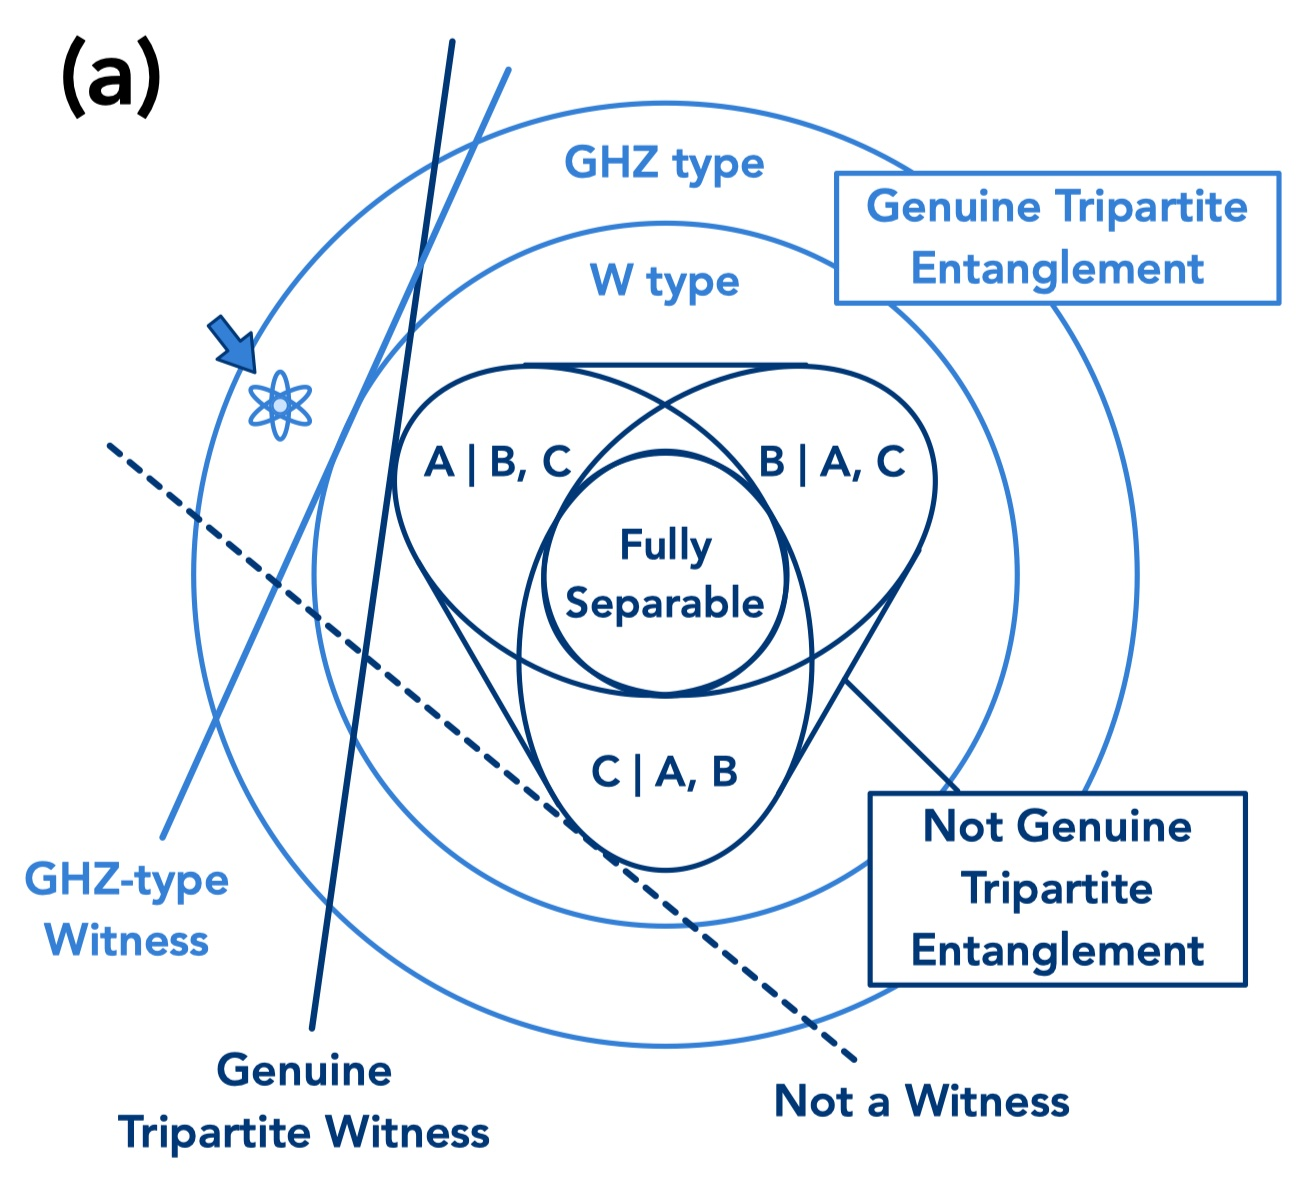
\includegraphics[width=.9\linewidth]{gme.jpg}
	\end{subfigure}
	\begin{subfigure}{0.3\textwidth}
		\centering
		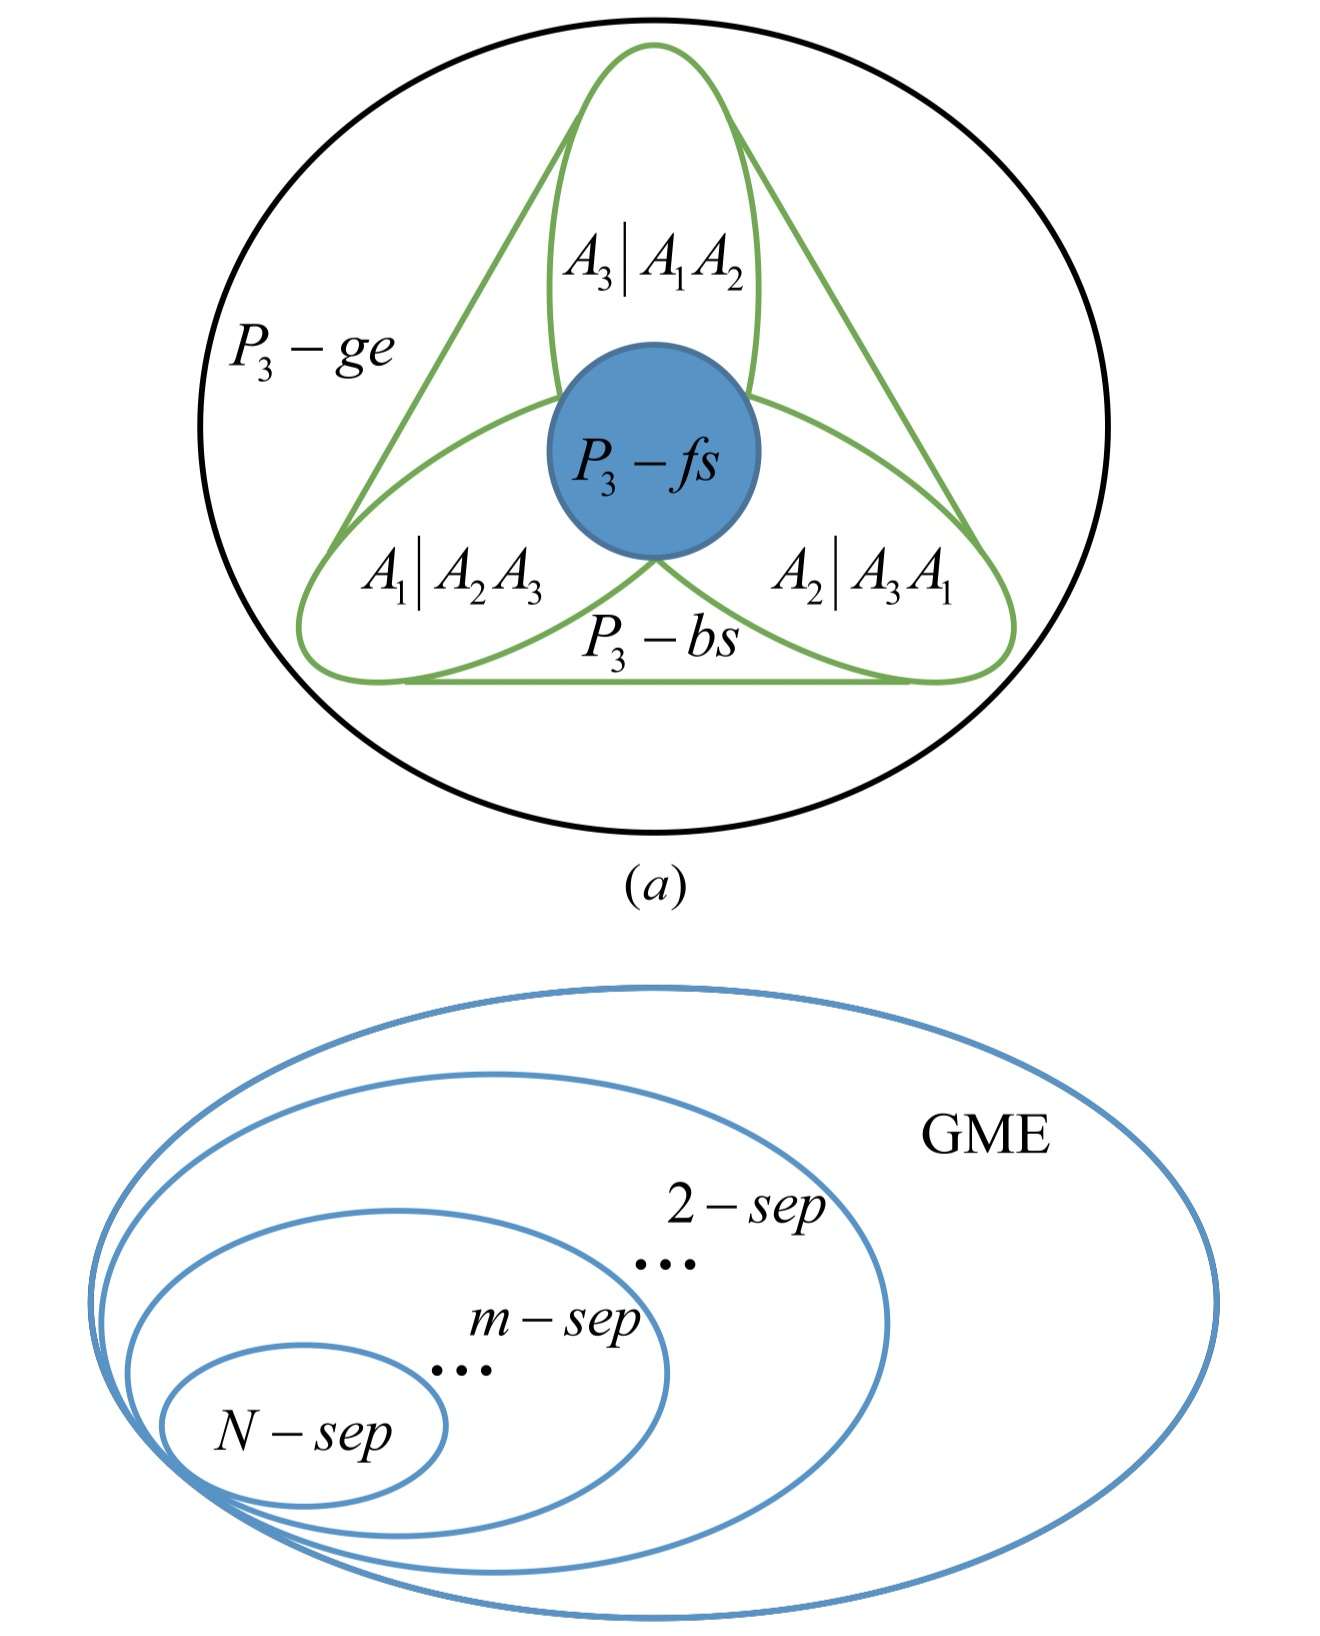
\includegraphics[width=.8\linewidth]{sep.jpg}
	\end{subfigure}
	\begin{subfigure}{0.3\textwidth}
		\centering
		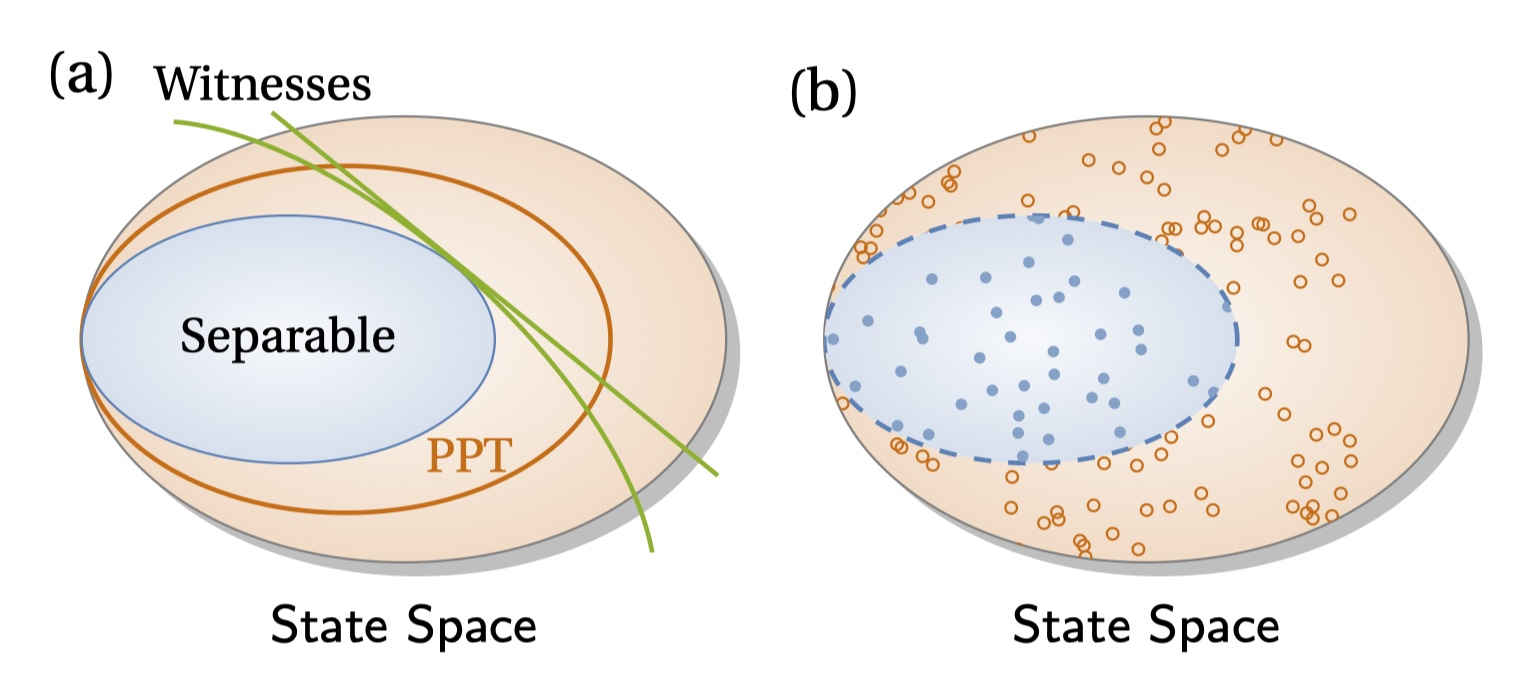
\includegraphics[width=.9\linewidth]{ppt.jpg}
	\end{subfigure}
	\caption{(a) entanglement witness, PPT criteria, SVM (kernel)?. (c) convex hull... }
	\label{fig:entangle}
\end{figure}

\subsubsection{Entanglement witness}\label{sec:entanglement_witness}
\begin{theorem}[\cite{gurvitsClassicalDeterministicComplexity2003}]
	% The problem of determining whether a given quantum state is entangled lies at the heart of quantum information processing, which is an NP-hard problem in general.
	The weak membership problem for the convex set of separable normalized bipartite density matrices is NP-Hard.
	\begin{itemize}
		\item \textbf{Input}: ??
		\item \textbf{Output}: ??
	\end{itemize}
\end{theorem}
\begin{question}
	specific cases? approximately correct? quantum computation? machine learning (data)?
\end{question}

\begin{theorem}[PPT criterion]
	the positive partial transpose (PPT) criterion, saying that a separable state must have PPT.
	Note, it is only necessary and sufficient when $d_A d_B \le 6$.
\end{theorem}
see \cref{fig:entangle}
\begin{definition}[entanglement witness]\label{def:entanglement_witness}
	Given an (unknown) quantum state (density matrix) $\dm$, the \emph{entanglement witness} $\ew$ is an obseverable such that
	\begin{equation}
		\Tr(\ew\dm) \ge 0 , \forall \text{ separable };\quad
		\Tr(\ew\dm) < 0 , \text{ for some entangled }
	\end{equation}
\end{definition}
It is natural to ask nonlinear entanglement witness \cite{guhneNonlinearEntanglementWitnesses2006}  
\nameref{def:kernel_method} ML

\begin{problem}[Entanglement witness with prior]
	% \cite{zhouDetectingMultipartiteEntanglement2019}
	with prior knowledge
	\begin{itemize}
		\item \textbf{Input}: a \textbf{known} state $\ket{\psi}$, with noise
		\item \textbf{Output}: ???
	\end{itemize}
	decision problem
\end{problem}

\subsubsection{Graph state}
graph state is an important class of multipartite states in quantum information.
Typical graph states include cluster states, \nameref{exm:ghz} state, and the states involved in error correction.
% cluster state is the special case of graph state.
2D cluster state is the universal resource for the measurement based quantum computation (MBQC) \cite{briegelMeasurementbasedQuantumComputation2009}.
\begin{definition}[graph state]\label{def:graph_state}
	Given a graph $G=(V,E)$, a graph state is constructed as 
	\begin{itemize}
		\item vertices: $\ket{+}^{\otimes n}$
		\item edges: apply controlled-Z to every edge,
		that is $\ket{G}=\prod_{(i,j)\in E}\textsf{cZ}_{(i,j)} \ket{+}^{\otimes n}$
	\end{itemize}
	An $n$-partite graph state can also be uniquely determined by $n$ independent stabilizers, 
	$S_i:= X_i \bigotimes_{j\in n}Z_j$, 
	which commute with each other and $\forall i,S_i\ket{G}=\ket{G}$.
\end{definition}
\begin{example}[graph states]
	GHZ; complete graph, hypercube, Petersen graph; cluster state
\end{example}
\begin{question}
	Hamiltona cycle of a graph state? vertex cover
\end{question}
% \begin{problem}[Entanglement structure detection]
% \end{problem}
\begin{problem}[Certify entanglement]
	Multipartite entanglement-structure detection
	\begin{itemize}
		\item \textbf{Input}: Given a state close to a \textbf{known} (general multipartite) state $\ket{\psi}$,
		certain partition?
		\item \textbf{Output}: the certified lower-order entanglement among several subsystems could be still useful for some quantum information tasks.
		entanglement structure
	\end{itemize}
\end{problem}
\begin{remark}
	The graph state is the unique eigenstate wtih eignevalue of +1 for all the $n$ stabilizers.
	As a result, a graph state can be writteb as a product of stailizer projectors, $\op{G}=\prod_{i=1}^n \frac{S_i +\identity}{2}$.
	stabilizer formalism?; 
\end{remark}
\begin{remark}
	The entanglement entropy $S( \dm_A )$ equals the rank of the adjacency matrix of the underlying bipartite graph, which can be efficiently calculated.
\end{remark}
\begin{proposition}[\cite{zhouDetectingMultipartiteEntanglement2019}]
	Given a graph state $\ket{G}$ and a partition $\mathcal{P}=\qty{A_i}$, the fidelity between $\ket{G}$ and any \nameref{def:fully_separable} is upper bounded by
	\begin{equation}
		\Tr(\op{G} \dm_f) \le \min_{\qty{A,\bar{A}}} 2^{-S(\dm_A)}
	\end{equation}
	where $S(\dm_A)$ is the von Neumann entropy of the reduced density matrix $\dm_A=\Tr_{\bar{A}}(\op{G})$.
\end{proposition}
\begin{theorem}
	k local measurements. Here, k is the chromatic number of the corresponding graph, typically, a small constant independent of the number of qubits.
\end{theorem}
\begin{proposition}[Entanglement of graph state]
	\cite{heinEntanglementGraphStates2006}.
	witness; bounds; graph property? vertex cover?
\end{proposition}
generalize \cite{zhangEfficientEntanglementGeneration2021}
stabilizer state, neural network state?


\subsection{Shadow tomography}
% \label{sec:shadow_tomography}
Intuitively, a general tomography \cite{altepeterPhotonicStateTomography2005} that extract all information about a state requires exponential copies (samples/measurements).
\begin{theorem}[lower bound of tomography?\cite{haahSampleOptimalTomographyQuantum}]
	Known fundamental lower bounds [66, 73] state that classical shadows of exponential size (at least) $T = \Omega( 2^n / \epsilon^2)$ are required to $\epsilon$-approximate $\dm$ in trace distance.
\end{theorem}
\begin{definition}[fidelity]\label{def:fidelity}
	Given a pair of states (target and real), 
	% \begin{equation}
	% 	F(\ket{\psi},\ket{\psi'}) :=
	% \end{equation}
	\begin{equation}
		F(\rho,\rho') : = \Tr \sqrt{\sqrt{\rho}\rho'\sqrt{\rho}}
	\end{equation}
	trace distance
	\begin{equation}
		d_{tr}(\rho,\rho') : = \frac{1}{2} \norm{\rho-\rho'}_1
	\end{equation}
	% relation
	% \begin{equation}
	% 	1-F\le D_{tr} \le \sqrt{1-F^2}
	% \end{equation}
\end{definition}
\begin{definition}[norm]\label{def:norm}
	Schatten p-norm $\norm{x}_p:= (\sum_i \abs{x_i}^p)^{1/p}$.
	Euclidean norm $l_2$ norm;
	Spectral (operator) norm ;
	Trace norm $\norm{A}_{tr}:=\Tr(\sqrt{A^\dagger A})$, $p=1$;
	Frobenius norm $\norm{A}_{tr}:=\sqrt{\Tr(A^\dagger A)}$, $p=2$;
	Hilbert-Schmidt norm
\end{definition}
\begin{problem}[Fidelity estimate]
	defined as follows
	\begin{itemize}
		\item \textbf{Input}: Given two density matrices $\dm$ and $\dm'$, 
		\item \textbf{Output}: \nameref{def:fidelity} with error $\epsilon$
	\end{itemize}
\end{problem}
\begin{problem}[Trace/expectaton estimate]
	defined as follows
	\begin{itemize}
		\item \textbf{Input}: Given an observable $\ob$ and a mixed state $\dm$ in density matrix,
		\item \textbf{Output}: the expectation value $\Tr(\ob \dm) = $ with error $\epsilon$ (trace distance)
	\end{itemize}
\end{problem}
Nevertheless, we usually only need specific property of a target state rather than all information about the state.
This enables the possibility to
Inspired by Aaronson's shadow tomography \cite{aaronsonShadowTomographyQuantum2018}, Huang et. al \cite{huangPredictingManyProperties2020}
\begin{problem}[Shadow tomography]\label{prm:shadow_tomography}
	\emph{shadow tomography}
	\begin{itemize}
		\item \textbf{Given (Input):} \textbf{unknown} $D$-dimensional mixed state $\rho$, known 2-outcome measurements $E_1,\dots,E_M$
		\item \textbf{Goal (Output):} estimate $\probability[E_i \text{ accept } \dm]$ to within additive error $\epsilon$, $\forall i\in [M]$, with $\ge 2/3$ success probability
	\end{itemize}
\end{problem}
\begin{theorem}[\cite{aaronsonShadowTomographyQuantum2018}]
	It is possible to do shadow tomography using $\tilde{\bigO}(\frac{\log^4 M\cdot \log D}{\epsilon^4})$ copies. [no construction algorithm?]
	sample complexity lower bound $\Omega(\log M\cdot \epsilon^{-2})$, 
\end{theorem}
random Pauli measurements
\begin{definition}[classical shadow]\label{def:classical_shadow}
	classical shadow
	\begin{equation}
		\dm_{cs} = \mathcal{M}^{-1} \qty(U^\dagger \op{\hat{b}} U)
	\end{equation}
\end{definition}
predict linear function with classical shadows
\begin{equation}
	o_i = \Tr(O_i \dm_{cs})
	\text{ obeys }
	\expectation[o] =\Tr(O_i \dm)
\end{equation}
The classical shadow attempts to approximate this expectation value by an empirical average over $T$ independent samples, much like Monte Carlo sampling approximates an integral.
% \begin{remark}
The classical shadow size required to accurately approximate all reduced $r$-body density matrices scales exponentially in subsystem size $r$, but is independent of the total number of qubits $n$.
% \end{remark}

\begin{algorithm}[H]
    \DontPrintSemicolon
    \SetKwInOut{Input}{input}
    \SetKwInOut{Output}{output}
    \Input{density matrix $\dm$, ..}
    \Output{classical shadow}
    \BlankLine
    \For{ $i = 1,2, \ldots, m$} {
        random Pauli measurements \tcp*{a comment}
        % \tcc{comment in a new line}
    {\Return "?"}
    }
    \Return ?
    \caption{Shadow tomography}
    \label{alg:classical_shadow}
\end{algorithm}
\begin{lemma}
	the variance
	\begin{equation}
		\variance[o] = \expectation[(o-\expectation[o])^2]
		\le \norm{O - \frac{\Tr(O)}{2^n} \identity}^2_{\shadow}
	\end{equation}
\end{lemma}
sample complexity
\begin{equation}
	N_{tot} = \bigO \qty(
		\frac{\log (M)}{\epsilon^2} \max_{1\le i\le M} 
		\norm{O_i - \frac{\Tr(O_i)}{2^n} \identity}^2_{\shadow}
	)
\end{equation}
\begin{theorem}[Pauli/Clifford measurements]
	additive error $\epsilon$, $M$ arbitrary $k$-local linear function $\Tr(\ob_i\dm)$,
	% lower bound
	$\Omega(\log(M) 3^k/\epsilon^2)$ copies of the state $\dm$.
\end{theorem}

\section{Classical, data-powered, and quantum algorithms}
We consider the problem 
\begin{problem}[???]
	problem without training data
	\begin{itemize}
		\item \textbf{Input}: a graph $\graph$ encoding in a graph state $\ket{\graph}$
		\item \textbf{Output}: entanglement structure
	\end{itemize}
	with training data
	\begin{itemize}
		\item \textbf{features}: classical shadow?
		\item label: 
	\end{itemize}
\end{problem}

\subsection{Quantum-classical (ML) hybrid method}
\subsubsection{Classical machine learning}\label{sec:classical_machine_learning}
separability classifier by neural network \cite{luSeparabilityEntanglementClassifierMachine2018}.
rigorous quantum advantage of quantum kernel method in SVM \cite{liuRigorousRobustQuantum2021}.
classical machine learning with \nameref{def:classical_shadow} \cite{huangProvablyEfficientMachine2021}.
\begin{definition}[SVM]
	find a hyperplane (a linear function)
\end{definition}
nonlinear boundary. map to a higher dimensional (feature) space, in which data is linearly separable.
\begin{definition}[kernel method]\label{def:kernel_method}
	Gaussian kernel; 
	graph kernel;
	shadow kernel
\end{definition}
\begin{figure}[!ht]
	\centering
	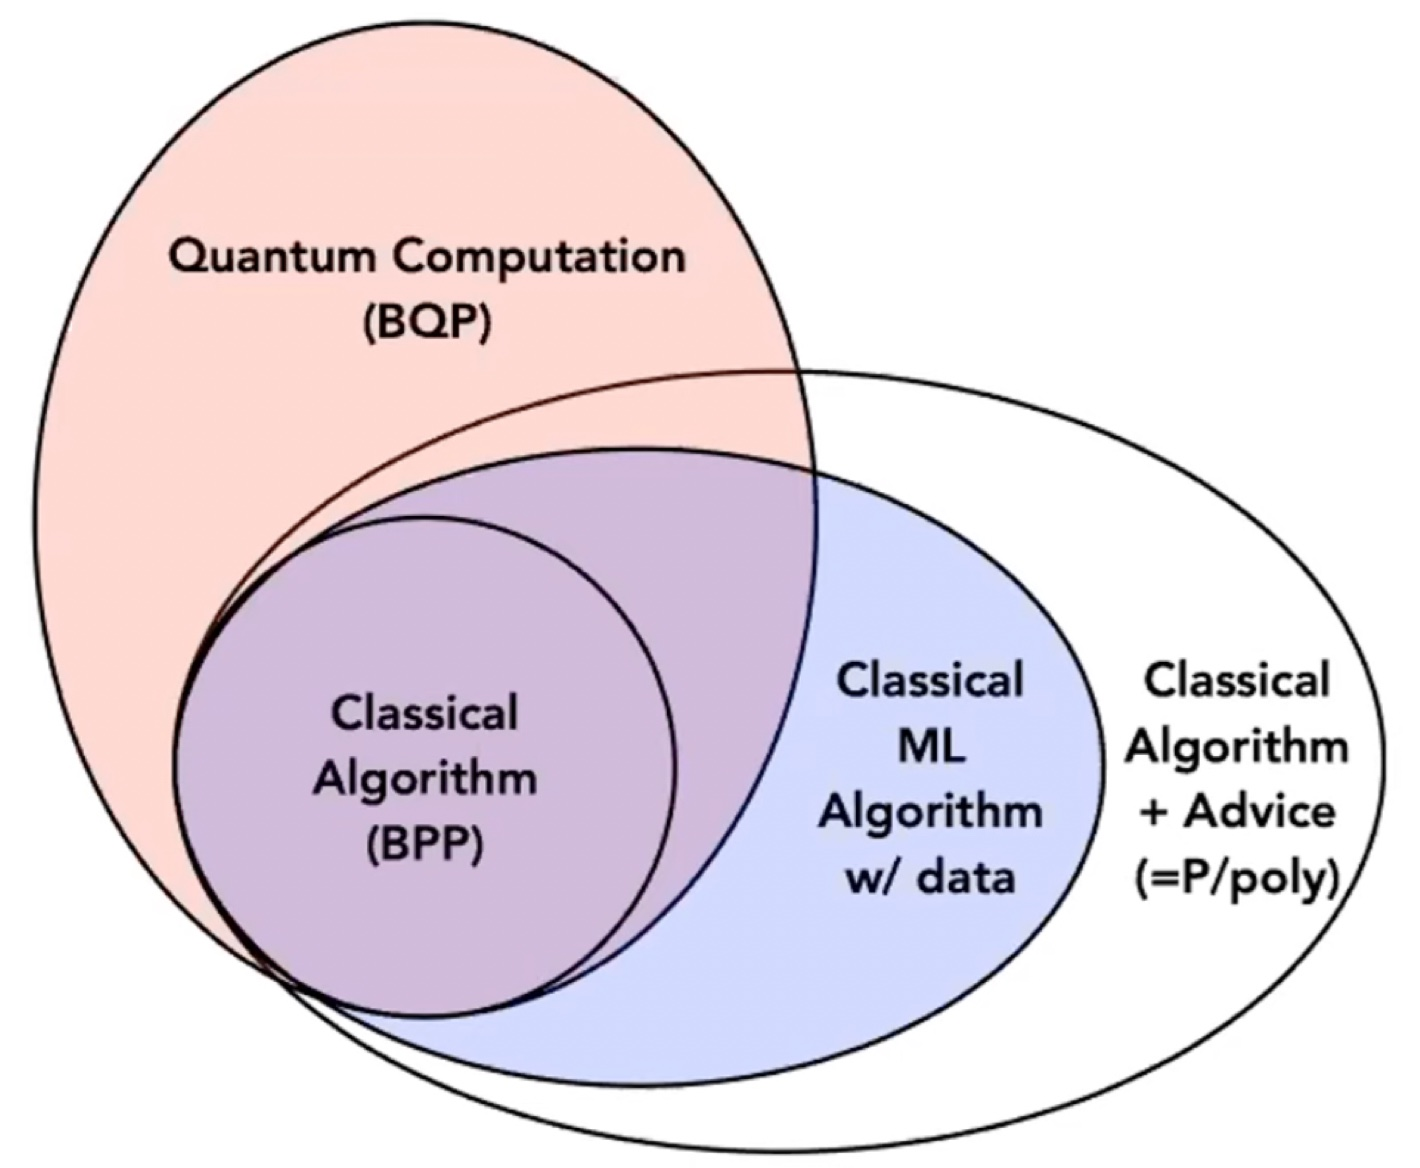
\includegraphics[width=.35\linewidth]{data.jpg}
	\caption{computational model powered by training data}
\end{figure}
\begin{theorem}[power of data]
	data learning
\end{theorem}
\begin{algorithm}[H]
    \DontPrintSemicolon
    \SetKwInOut{Input}{input}
    \SetKwInOut{Output}{output}
    \Input{labeled features (data)}
    \Output{entanglement structure}
    \BlankLine
    \For{ $i = 1,2, \ldots, m$} {
        kernel estimation \tcp*{a comment}
        % \tcc{comment in a new line}
    {\Return "?"}
    }
    \Return ?
    \caption{Classical learning (SVM)}
    \label{alg:classical_learning}
\end{algorithm}

\subsubsection{Quantum trace estimation and kernel estimation}
The task of estimating quantities like 
\begin{equation}
	\Tr(\rho_1 \cdots \rho_m)
	\tag{multivariate traces}
\end{equation}
given access to copies of the quantum states $\rho_1$  through $\rho_m$.
% is a fundamental building block in quantum information science
\begin{theorem}[Quantum trace estimation]
	\cite{quekMultivariateTraceEstimation2022}
	multivariate trace estimation can be implemented in constant quantum depth, with only linearly-many controlled two-qubit gates and a linear amount of classical pre-processing	
\end{theorem}

\subsection{Variational quantum circuits}
\subsubsection{Variational quantum kernel estimation}
an ansatz
\begin{equation}
	\ew_{a} := \sum_i  a_{..} \bigotimes \hat{\sigma}^{(n)}
	,\quad \hat{\sigma} \in \qty{\sx,\sy,\sz,I}
\end{equation}
\begin{algorithm}[H]
    \DontPrintSemicolon
    \SetKwInOut{Input}{input}
    \SetKwInOut{Output}{output}
    \Input{density matrix $\dm$}
    \Output{determine entangled structure??}
    \BlankLine
    \For{ $i = 1,2, \ldots, m$} {
        $W_i$  \tcp*{this is a comment}
        % \tcc{comment in a new line}
    {\Return "separable?"}
    }
    \Return entangled ?
    \caption{Entanglement witness by ...}
    \label{alg:entanglement_witness}
\end{algorithm}

\subsubsection{Variational trace estimate}
find optimal entanglement witness (qunatum circuit?)
\cite{glickCovariantQuantumKernels2021}
% \cite{liuRigorousRobustQuantum2021}
\cite{havlicekSupervisedLearningQuantum2019}
\cite{schuldQuantumMachineLearning2019}

\subsection{Theoretic upper bounds and lower bounds}
\cite{huangPowerDataQuantum2021}
\cite{huangPredictingManyProperties2020}
\cite{aaronsonShadowTomographyQuantum2018}
\cite{huangInformationtheoreticBoundsQuantum2021}
\cite{liuRigorousRobustQuantum2021}
\begin{definition}[graph property]\label{def:graph_property}
	monotone
\end{definition}
\begin{problem}[Graph property test]
\end{problem}
quantum advantages:
\begin{itemize}
	\item no input encoding problem \cite{tangQuantumPrincipalComponent2021} in most quantum machine learning algorithm.
	\item contrived problem? for exponential speedup
	\item convex body query? complexity
\end{itemize}
obstacles: (i)
\begin{table}[!ht]
\centering
\begin{tabular}{c|c|c|c|c}
	& gate/depth/computation & query?complexity & measurements/samples & necessary/sufficient \\  
	\hline
	\nameref{prm:shadow_tomography}:  & & N/A & $\bigO$, Holevo bound $\Omega$ & \\  
	indirect? direct (no prior) & & & & \\  
	promise (low-rank?), partial, decision? & & & & \\  
	entanglement witness (\cref{sec:entanglement_witness}) & & & constant & \\  
	classical ML (\cref{sec:classical_machine_learning})  & & & & \\  
	quantum (variational) circuits & c-depth? & & & \\  
	\hline
\end{tabular}
\caption{complexity measures of different methods}
\end{table}

\section{Numerical simulation}
\subsection{Classification accuracy}
\subsubsection{Data preparation}
generate synthetic data from

\subsubsection{Results}
performance of different methods: 
% \begin{itemize}
% 	\item shadow tomography: 
% 	\item entanglement witness (no machine learning); 
% 	\item classical machine learning; 
% 	\item quantum machine learning
% \end{itemize}

\subsection{Robustness to noise}
tradeoff between (white noise) tolerance (robustness) and efficiency (number of measurements).
\begin{equation}
	\dm_{\noise}' = (1-p_{\noise}) \op{G} + p_{\noise} \frac{\identity}{2^n}
\end{equation}
$p_{noise}$ indicates the robustness of the algorithm (witness).
\begin{remark}
	the largest noise tolerance $p_{limit}$ just related to the \textbf{chromatic number} of the graph.[??]
	\nameref{def:graph_property}
\end{remark}
% \input{complexity.tex}
% \input{optimization.tex}

\section{Conclusion and discussion}
todo
\begin{itemize}
	\item experiment (generation, verification) \cite{luEntanglementStructureEntanglement2018}
	\item error correction? not benchmark
\end{itemize}

\subsection*{Acknowledgements}
% \thanks{The author thanks} 
% The author thanks
% TikZiT, QuTip

%\begin{appendices}
    %\chapter{}
%\end{appendices}

% %%%%%%%%%%%%%%%Reference%%%%%%%%%%%%%%%
% % \newpage
% % \printbibliography
\bibliographystyle{apsrev4-2}
%\bibliographystyle{alpha}
\bibliography{ref}

%\begin{widetext}
\onecolumngrid
\appendix

\section{Machine learning background}
% In this work, we restrict ourself to supervised learning (mainly SVM), where we are given a set of labeled data for training to predict labels of new data.
% \subsection{SVM}
% \subsection{neural network}
% \subsection{Unsupervised: PCA}

%\end{widetext}

\end{document}